%ARCHITETTURA APP ESTERNA
\subsection{Applicazione esterna alla piattaforma Grafana}
Per poter visualizzare la suddivisione delle componenti dell'applicazione esterna e le dipendenze che sussistono tra loro ad alto livello, viene riportato il diagramma dei Package in allegato nel file \textit{diagramma-package-app.png}.
	\subsubsection{Progettazione architetturale}
	Abbiamo deciso di utilizzare un design pattern architetturale Model-View-ViewModel (MVVM) perché si adatta bene alle tecnologie che vengono utilizzate ovvero React ed Electron. In particolare, come si può vedere dalla figura seguente, la View invia dati a ViewModel che a sua volta fornisce delle risposte che permettono di tenere la vista sempre aggiornata. Questo scambio di dati è asincrono ed è fornito interamente da Electron. Inoltre abbiamo la comunicazione tra ViewModel e Model che avviene con la richiesta di esecuzione delle operazioni da parte del ViewModel ed la conseguente risposta da parte del Model. Anche questo scambio di messaggi è asincrono ed è implementato da un meccanismo di callback.
	%\mbox{}
	%\begin{landscape}
	%	\begin{figure}
	%		\begin{figure} [H]
	%			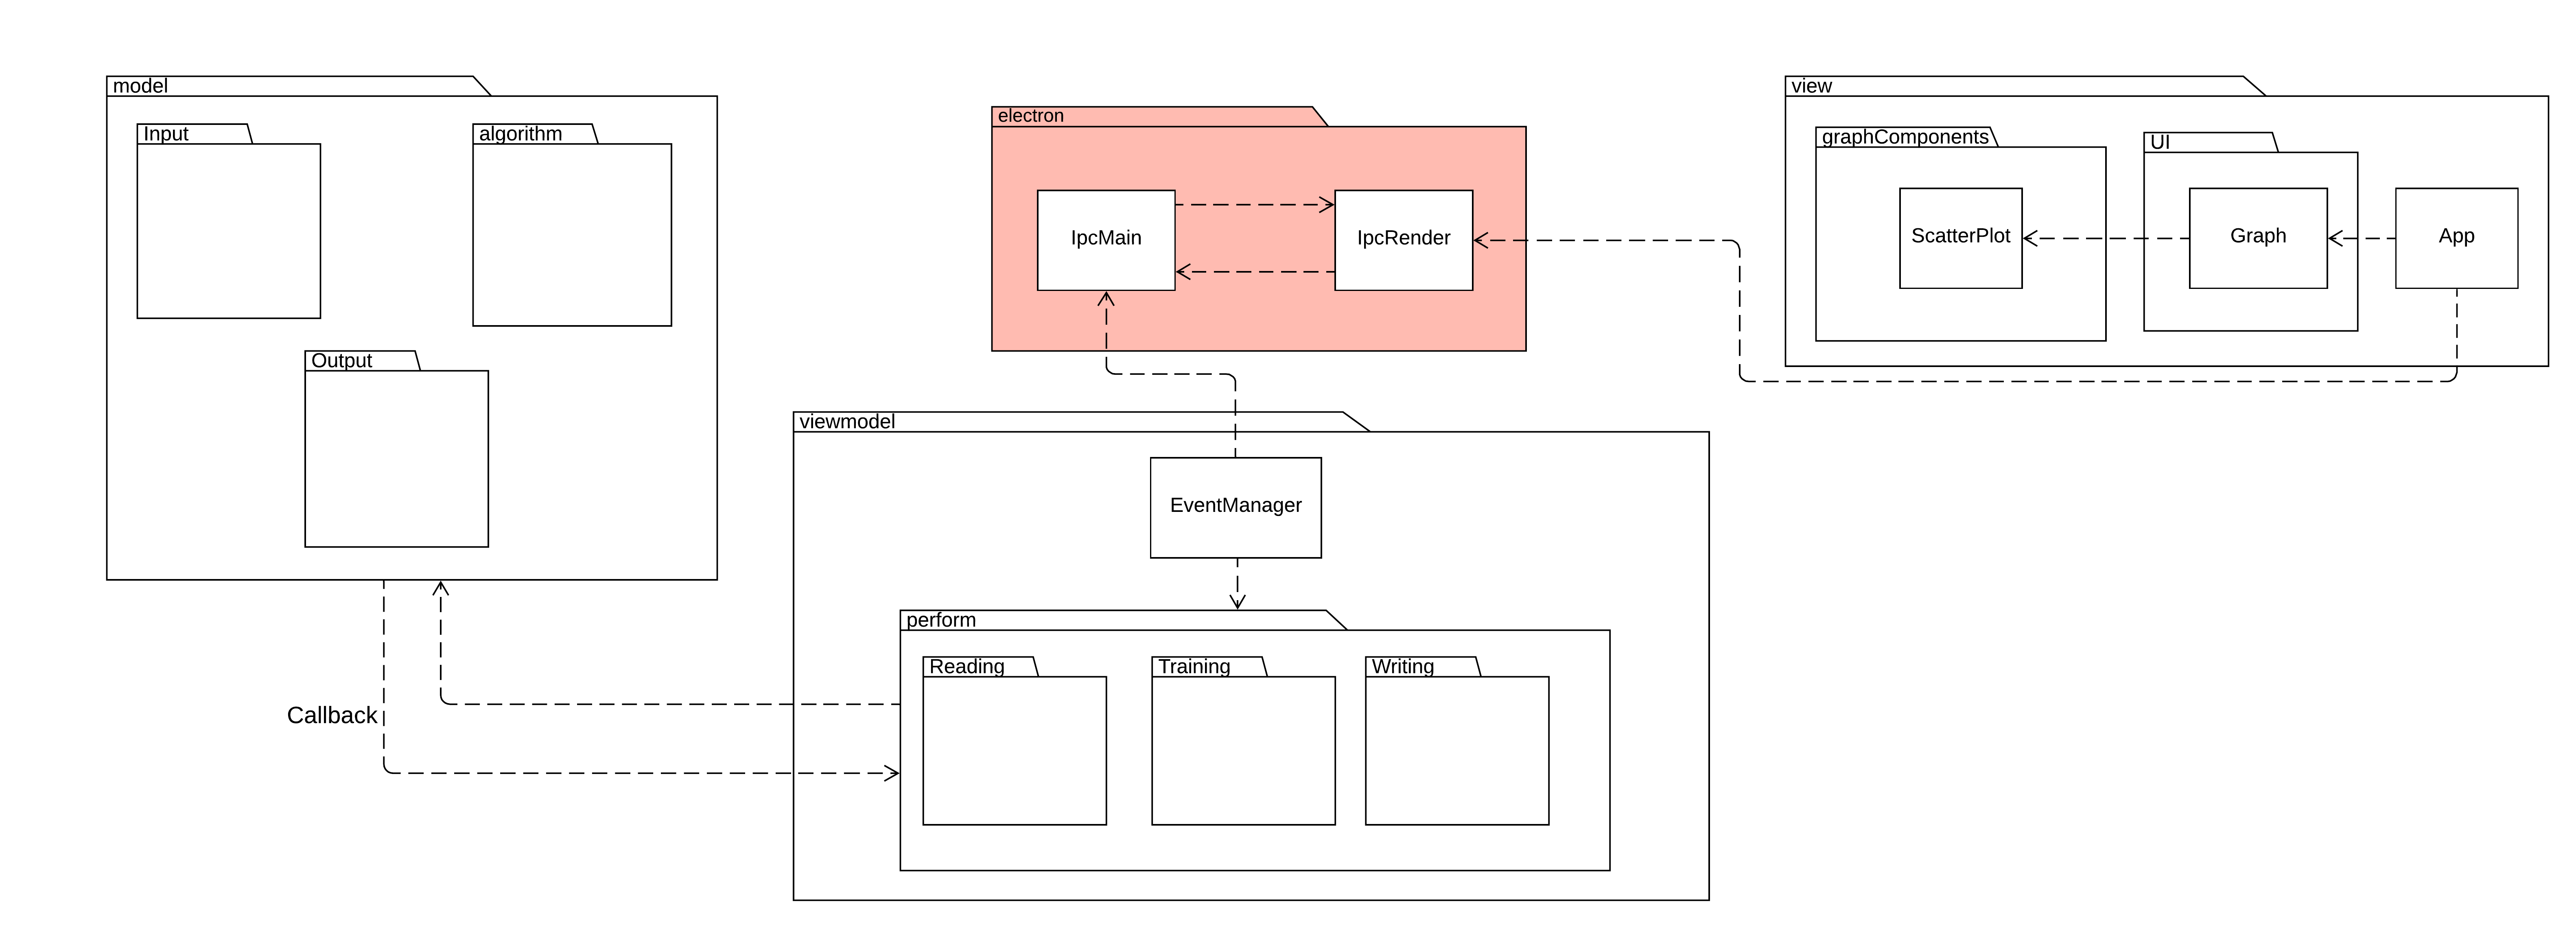
\includegraphics[width=\linewidth]{./img/Diagrammi/architettura-app.png}
	%			\caption{Diagramma dell'architettura dell'applicazione}
	%		\end{figure}
	%	\end{figure}
	%\end{landscape}
	Analizzando i componenti, la nostra architettura è così strutturata: 
	\begin{itemize}
		\item \textbf{Model}: modulo che gestisce la business logic. Più in dettaglio esegue l'addestramento dei dati attraverso gli algoritmi di predizione e le operazioni di input/output dei file;
		\item \textbf{View}: modulo che gestisce la presentazione dei dati attraverso React;
		\item \textbf{ViewModel}: modulo che gestisce il binding tra View e Model con un meccanismo detto two-way-data-binding.
	\end{itemize}
	\subsubsection{Progettazione di dettaglio}
		Di seguito viene descritta in dettaglio la progettazione dell'applicazione. In allegato viene fornito il file \textit{diagramma-classi-app.png} contenente l'intero diagramma delle classi.
		\paragraph{Model} \mbox{}
		\paragraph*{Read} \mbox{}
		Abbiamo riscontrato che nella gestione dell'input, indipendentemente dalla tipologia di file ricevuto, l'algoritmo per eseguire la lettura di quest'ultimo ha uno scheletro comune. È stato quindi deciso di implementare il design pattern template method.
		La classe astratta \textit{Read} implementa il metodo \textit{ReadFile(path, callback)} che rappresenta la parte comune dell'algoritmo di lettura da file. Inoltre presenta il metodo astratto \textit{parser(data, callback)} che invece rappresenta la trasformazione del contenuto del file sulla base della sua estensione e perciò viene implementato nelle classi concrete che estendono \textit{Read}. Nel nostro caso esse sono \textit{ReadCsv} e \textit{ReadJson}.
		%INSERIRE IMMAGINE READ APP
		\paragraph*{Write} \mbox{}
		Anche nella gestione dell'output abbiamo riscontrato che, indipendentemente dalla tipologia di file su cui scrivere, l'algoritmo per eseguire la scrittura di quest'ultimo ha uno scheletro comune. È stato quindi deciso di implementare il design pattern template method.
		La classe astratta \textit{Write} implementa il metodo \textit{writeToDisk(path, name, data)} che rappresenta
		\paragraph{View} \mbox{}
		\paragraph{ViewModel} \mbox{}